\documentclass{article}
\usepackage{amsmath,amsfonts,amsthm,amssymb,amsopn,bm}
\usepackage[margin=.9in]{geometry}
\usepackage{graphicx}
\usepackage{url}
\usepackage[usenames,dvipsnames]{color}
\usepackage{fancyhdr}
\usepackage{multirow}
\usepackage{listings}
\usepackage{hyperref}

\definecolor{keywords}{RGB}{255,0,90}
\definecolor{comments}{RGB}{0,0,113}
\definecolor{red}{RGB}{160,0,0}
\definecolor{green}{RGB}{0,150,0}
 
\lstset{language=Python, 
        basicstyle=\ttfamily\tiny, 
        keywordstyle=\color{keywords},
        commentstyle=\color{comments},
        stringstyle=\color{red},
        showstringspaces=false}

\newcommand{\field}[1]{\mathbb{#1}}
\newcommand{\1}{\mathbf{1}}
\newcommand{\E}{\mathbb{E}} 
\newcommand{\Z}{\mathbb{Z}} 
\renewcommand{\P}{\mathbb{P}}
\newcommand{\R}{\field{R}} % real domain
% \newcommand{\C}{\field{C}} % complex domain
\newcommand{\F}{\field{F}} % functional domain
\newcommand{\T}{^{\textrm T}} % transpose
\def\diag{\text{diag}}

%% operator in linear algebra, functional analysis
\newcommand{\inner}[2]{#1\cdot #2}
\newcommand{\norm}[1]{\left\|#1\right\|}
\newcommand{\twonorm}[1]{\|#1\|_2^2}
% operator in functios, maps such as M: domain1 --> domain 2
\newcommand{\Map}[1]{\mathcal{#1}}
\renewcommand{\theenumi}{\alph{enumi}} 

\newcommand{\Perp}{\perp \! \! \! \perp}

\newcommand\independent{\protect\mathpalette{\protect\independenT}{\perp}}
\def\independenT#1#2{\mathrel{\rlap{$#1#2$}\mkern2mu{#1#2}}}
\newcommand{\vct}[1]{\boldsymbol{#1}} % vector
\newcommand{\mat}[1]{\boldsymbol{#1}} % matrix
\newcommand{\cst}[1]{\mathsf{#1}} % constant
\newcommand{\ProbOpr}[1]{\mathbb{#1}}
\newcommand{\points}[1]{\small\textcolor{magenta}{\emph{[#1 points]}} \normalsize}
\date{{}}

\setlength\parindent{0px}
\makeatletter
\DeclareUrlCommand\ULurl@@{%
  \def\UrlFont{\ttfamily\color{blue}}%
  \def\UrlLeft{\uline\bgroup}%
  \def\UrlRight{\egroup}}
\def\ULurl@#1{\hyper@linkurl{\ULurl@@{#1}}{#1}}
\DeclareRobustCommand*\ULurl{\hyper@normalise\ULurl@}
\makeatother

%\newcommand{\ind}{\mbox{$~\underline{~\parallel~}~$}}%
\newcommand{\ind}{\mbox{$\perp \kern-5.5pt \perp$}}
\newcommand{\nind}{\mbox{$\not\hspace{-4pt}\ind$}}


\begin{document}
\title{Homework \#8}
\author{\normalsize{Winter 2020, STATS 509}\\
\normalsize{Dino Bektesevic}}
\maketitle

\subsection*{Problem 1: Properties of Estimators and Confidence Intervals}
Goldberger Qu. 11.2\par
 {\it Hints: For (a) use common sense / the analogy principle; for (b) read Goldberger \S 10.1, p.107; for part (c) use the analogy principle and p.108; for (d) recall that the standard error of $T$ is simply an estimate of the standard deviation of $T$.\footnote{This usage of the term `standard error' follows Goldberger (p.123) who defines the `standard error' of $\bar{Y}$ to be $s/\sqrt{n}$ which is an {\bf estimate} of $\sigma/\sqrt{n}$, the standard deviation of $\bar{Y}$. (Here assuming $\sigma$ is unknown.\par
  However, other authors use `standard error of $\bar{Y}$' to refer to $\sigma/\sqrt{n}$; such authors will then refer to $s/\sqrt{n}$ as an {\bf estimated} standard error.
(For Goldberger, adding the word `estimated' to `standard error' would be redundant.)}}
\begin{enumerate}
    \item We can pick $T=\bar X - \bar Y$ since:
    $$E[T] = E[\bar X] - E[\bar Y] = \mu_X - \mu_Y = \theta$$
    
    \item 
    \begin{align*}
        V(T) &= Cov(T, T) = Cov(\bar X - \bar Y, \bar X - \bar Y) \\
        &= V(\bar X) + V(\bar Y) - 2Cov(\bar Y, \bar X ) \\
        &= V(\bar X) + V(\bar Y) - 2Cov\left(\frac{1}{n}\sum_i^n y_i, \frac{1}{n}\sum_i^n x_i \right) \\
        &= V(\bar X) + V(\bar Y) - \frac{2}{n^2} \sum_{i,j=1}^n Cov(y_i, x_j) \\
        &= V(\bar X) + V(\bar Y) - \frac{2}{n^2} \sum_{i,j=1}^n \sigma_{XY}\\
        &= \frac{\sigma^2_X}{n} + \frac{\sigma^2_Y}{n} - \frac{2}{n^2} n \sigma_{XY} \\
        &= \frac{\sigma^2_X + \sigma^2_Y - 2\sigma_{XY}}{n} 
    \end{align*}
    
    \item By analogy with b) we can just say:
    $$V(T) =  \frac{S^2_X + S^2_Y - 2S_{XY}}{n} $$
    but following Goldberger's definitions of these values to make them unbiased:
    $$V(T) =  \frac{\frac{n}{n-1}S^2_X + \frac{n}{n-1}S^2_Y - 2\frac{n}{n-1}S_{XY}}{n} = \frac{S^2_X + S^2_Y - 2S_{XY}}{n-1}  $$
    
    \item For standard error of T I would report $\sqrt{V(T)}$
\end{enumerate}


\newpage
\subsection*{Problem 2}
Goldberger Qu. 11.3
 {\it Hints: see p.119. For part (a), express the estimator as $T=a_1{\bar{Y}_1} +a_2{\bar{Y}_2}$; find a constraint on $a_1$ and $a_2$ in order for $T$ to be unbiased for $\mu$; use this to solve for $a_2$ in terms of $a_1$; find the variance of $T$; substitute for $a_2$, and then differentiate the variance with respect to $a_1$.}
 \begin{enumerate}
     \item We are asked to consider $T=c_1\bar Y_1 + c_2 \bar Y_2$. We want it to be unbiased so:
     
     $$ \mu = E[T] = c_1 E[\bar Y_1] + c_2 E[\bar Y_2] = c_1\mu + c_2\mu = (c_1 + c_2)\mu  $$
     
     we must conclude that $c_1 + c_2 = 1 = \rightarrow c_2 = 1-c_1$ if unbiased-ness is to hold true. We are asked to find the minimum variance unbiased estimator so:
     \begin{align*}
         V(T) &= V(c_1\bar Y_1 + c_2 \bar Y_2) \\
         &= V(c_1\bar Y_1) + V(c_2 \bar Y_2) \\
         &= c_1^2 V(\bar Y_1) + c_2^2 V(\bar Y_2) \\
         &=  c_1^2 V(\bar Y_1) + (1-c_1)^2 V(\bar Y_2) 
     \end{align*}
     where we, in line 2, used the fact that the problem tells us that the two samples are independent so $Cov(\bar Y_1, \bar Y_2)=0$. We minimize the variance as a function of the constants:
    \begin{align*}
        0 &= \frac{\partial}{\partial c_1} V(T)  \\
        0 &= \frac{\partial}{\partial c_1} \left( c_1^2 V(\bar Y_1) + (1-c_1)^2 V(\bar Y_2)  \right) \\
        0 &= 2c_1 V(\bar Y_1) - 2(1-c_1)V(\bar Y_2) \\
        0 &= 2c_1( V(\bar Y_1) + V(\bar Y_2) ) - 2V(\bar Y_2) \\
        c_1 &= \frac{V(\bar Y_2)}{V(\bar Y_1) + V(\bar Y_2)} \\
        &\rightarrow c_2 = 1 - c_1 = \frac{V(\bar Y_1)}{V(\bar Y_1) + V(\bar Y_2)}
    \end{align*}
    We verify that this is the minimum:
    \begin{align*}
        \frac{\partial^2}{\partial c_1^2} V(T) &= \frac{\partial}{\partial c_1}   2c_1( V(\bar Y_1) + V(\bar Y_2) ) - 2V(\bar Y_2) = 2( V(\bar Y_1) + V(\bar Y_2) ) \geq 0
    \end{align*}
    since variance is always positive or zero.
    
     \item to verify that $V(T) < V(\bar Y_1), V(\bar Y_2)$ we can write: 
     \begin{align*}
        V(T) &=  V(c_1\bar Y_1 + c_2 \bar Y_2) \\
        &= \left(\frac{V(\bar Y_2)}{V(\bar Y_1) + V(\bar Y_2)}\right)^2 V(\bar Y_1)  +  \left(\frac{V(\bar Y_1)}{V(\bar Y_1) + V(\bar Y_2)} \right)^2 V(\bar Y_2) \\
        &= \frac{V(\bar Y_2)^2 V(\bar Y_1) + V(\bar Y_1)^2V(\bar Y_2)}{\left(V(\bar Y_1) + V(\bar Y_2)\right)^2} \\
        &= \frac{V(\bar Y_1)V(\bar Y_2)\left(V(\bar Y_2) + V(\bar Y_1)\right)}{\left(V(\bar Y_1) + V(\bar Y_2)\right)^2} \\
        &= \frac{V(\bar Y_1)V(\bar Y_2)}{V(\bar Y_1) + V(\bar Y_2)} 
    \end{align*}
    To show the inequality we can write
    \begin{align*}
        \frac{V(T)}{V(\bar Y_1)} &= \frac{V(\bar Y_2)}{V(\bar Y_1) + V(\bar Y_2)} \leq 1 \\
        \frac{V(T)}{V(\bar Y_2)} &= \frac{V(\bar Y_1)}{V(\bar Y_1) + V(\bar Y_2)} \leq 1 
    \end{align*}
 \end{enumerate}
 


\newpage
\subsection*{Problem 3}
Goldberger Qu. 11.4. Assume that $Y_1$ and $Y_2$ are independent.

We are told that we have $N=100$ samples where $n_1$ comes from $Y_1\sim N(\mu_1, 50)$ and $n_2$ comes from $Y_2\sim N(\mu_2, 100)$ so that $N=n_1+n_2$. 

We are estimating $T=\mu_1 - \mu_2$ just like in question 1 so we can use $T=\bar Y_1 - \bar Y_2$ as an unbiased estimator of $\theta$. To get the best estimation of $\theta$ we want to minimize the variance of T. So we can write:
\begin{align*}
    V(T) &= V(\bar Y_1) + V(\bar Y_2) \\
    &= \frac{\sigma^2_1}{n_1} + \frac{\sigma^2_2}{n_2} \\
    &= \frac{\sigma^2_1}{n_1} + \frac{\sigma^2_2}{N - n_1}
\end{align*}
Where we used the fact $Y_1$ and $Y_2$ are independent. Minimizing this expression with respect to number of samples $n_1$ will tell us how many samples of $Y_1$ we want to get the best estimate of $\theta$: 
\begin{align*}
    \frac{\partial}{\partial n_1} V(T) &=  \frac{\partial}{\partial n_1} \left[ \frac{\sigma^2_1}{n_1} + \frac{\sigma^2_2}{N - n_1} \right] = 0 \\
    -\frac{\sigma^2_1}{n_1^2} + \frac{\sigma^2_2}{(N - n_1)^2} &= 0\\
    \sigma^2_1 (N-n_1)^2 &= \sigma^2_2 n_1^2 \\
    \sigma^2_2 n_1^2 - \sigma^2_1 (N^2 -2Nn_1 + n_1^2) &= 0\\
    \sigma^2_2 n_1^2 - \sigma^2_1 N^2 + 2\sigma^2_1 Nn_1 - \sigma^2_1 n_1^2 &= 0\\
    (\sigma^2_2 - \sigma^2_1) n_1^2 + 2\sigma^2_1 Nn_1 - \sigma^2_1 N^2  &=0 \\
    \left(\frac{\sigma^2_2}{\sigma^2_1} - 1\right) n_1^2 + 2Nn_1 - N^2  &=0 \\
    \left(\frac{100}{50} - 1\right) n_1^2 + 200n_1 - 10000  &=0 \\
    n_1^2 + 200n_1 - 10000  &=0 \\
    \rightarrow &n_{1,1} = 41.42\\
    &n_{1,2} = -241.42
\end{align*}
So we would want to draw 41 sample from $Y_1$ and 59 from $Y_2$. We can verify that this is a minimum:

\begin{align*}
    \frac{\partial^2}{\partial n_1^2} V(T) &=  \frac{\partial}{\partial n_1} \left[\left(\frac{\sigma^2_2}{\sigma^2_1} - 1\right) n_1^2 + 2Nn_1 - N^2 \right]  \\
    &= 2\left(\frac{\sigma^2_2}{\sigma^2_1} - 1\right) n_1|_{n_1=41.42} + 2N   \\
    &= 2 n_1|_{n_1=41.42} + 200 = 282.84 > 0   \\
\end{align*}



\newpage
\subsection*{Problem 4: Maximum Likelihood / ZES Estimation / GLRTs}
Suppose that $X_1,\ldots ,X_n$ are i.i.d.~observations from the following pmf:
$$ f(x \mid \theta)  = \left\{\begin{array}{cl}
        \left. e^{\theta x}\right/\left(1+e^{\theta}\right) & x \in \{0,1\} \\[4pt]
        0 & \hbox{otherwise}
        \end{array}
        \right.
$$
where $\theta \in \mathbb{R}$.
\begin{enumerate}
    \item Confirm that for any value of $\theta$, this is a probability mass function.
    
    \begin{align*}
        \sum_x f(x|\theta) &= 1 \\
        f(0|\theta) + f(1|\theta) &= 1\\
        \frac{1}{1+e^\theta}  + \frac{e^\theta}{1+e^\theta} &= 1 \\
        \frac{1+e^\theta}{1+e^\theta} &= 1 \,\,\, \forall \theta \in \R
    \end{align*}
    
    \item Write down the likelihood for one observation $f(x \mid \theta)$. Find the log-likelihood, $\ell = \log f(x \mid \theta)$.
    
    Following the example in Goldberger 12.2, p 130:
    \begin{align*}
        L(\theta |x) &= \left(\frac{e^\theta}{1+e^\theta}\right)^x \left(\frac{1}{1+e^\theta}\right)^{1-x} \\
        l(\theta|x) &= \ln{\left( \frac{e^{\theta x}}{1+e^\theta}   \right)} = \ln{e^{\theta x}} - \ln{(1+e^\theta)} \\
        &= x\theta - \ln{(1+e^\theta)}
    \end{align*}
    
    \item Find the score variable $Z = ({\partial\ell / \partial \theta})$. Using the fact that $E[Z]=0$, find $E(X)$ (see Goldberger p.128). 
    
    The score variable is:
    $$Z = \frac{\partial}{\partial\theta} l(\theta | x) = x - \frac{e^\theta}{1+e^\theta} $$
    and its expectation value:
    \begin{align*}
        E[Z] &= E\left[ x - \frac{e^\theta}{1+e^\theta} \right] \\
        0 &= E[x] - \frac{e^\theta}{1+e^\theta} \\
        E[X] &= \frac{e^\theta}{1+e^\theta}
    \end{align*}
    
    \newpage
    \item Find the maximum likelihood estimator $\hat{\theta}$ of $\theta$ based on the random sample $X_1,\ldots , X_n$.
    
    \begin{align*}
       0 &= \frac{\partial }{\partial\theta} \ln l(\theta | x_1,\hdots,x_n) \\
       0 &= \frac{\partial }{\partial\theta} \ln \prod_i^n l(\theta | x_i) \\
       0 &= \frac{\partial }{\partial\theta} \sum_i^n \ln l(\theta | x_i) \\
       0 &= \sum_i^n \frac{\partial }{\partial\theta}  \ln l(\theta | x_i) \\
       0 &= \sum_i^n \frac{\partial }{\partial\theta}  x_i\theta - \ln{(1+e^\theta)} \\
       0 &= \sum_i^n x_i - \frac{e^\theta}{1+e^\theta} \\
       \frac{ne^\theta}{1+e^\theta} &= \sum_i^n x_i \\
       ne^\theta &= \sum_i^n x_i + e^\theta\sum_i^n x_i \\
       \left(n - \sum_i^n x_i\right) e^\theta &= \sum_i^n x_i \\
       \theta_{MLE} &= \ln{\left( \frac{\sum_i^n x_i}{n - \sum_i^n x_i} \right)  } \\
       \theta_{MLE} &= \ln{\left( \frac{n\bar x}{n - n\bar x} \right)  } \\
       \theta_{MLE} &= \ln{\left( \frac{\bar x}{1 - \bar x} \right)  } \\
    \end{align*}
    We can verify this is a maximum:
    \begin{align*}
       \frac{\partial^2 }{\partial\theta^2} \ln l(\theta | x_1,\hdots,x_n) &= \frac{\partial }{\partial\theta}  \sum_i^n x_i - \frac{e^\theta}{1+e^\theta} = -n \frac{\partial }{\partial\theta} \frac{e^\theta}{1+e^\theta}  \\
        &= -n\left(e^\theta \frac{\partial}{\partial\theta} \frac{1}{1+e^\theta}  +  \frac{1}{1+e^\theta} \frac{\partial}{\partial\theta} e^\theta \right) \\
        &= -n\left(e^\theta \frac{-1}{(1+e^\theta)^2}e^\theta  +  \frac{1}{1+e^\theta} e^\theta \right) \\
        &= -n\left(\frac{-e^{2\theta}}{(1+e^\theta)^2}  +  \frac{e^\theta}{1+e^\theta}  \right) \\
        &= -n\left(\frac{-e^{2\theta} + (1+e^\theta)e^\theta}{(1+e^\theta)^2} \right) \\
        &= -\frac{ne^\theta}{(1+e^\theta)^2} < 0    
    \end{align*}
    No need to evaluate at $\theta_{MLE}$ this will always be negative. 
    
    
    \newpage
    \item Derive the ZES estimator for $\theta$. Confirm that this leads to the same estimator for $\theta$ that you obtained in (d).
    
    By definition:
    
    \begin{align*}
        \frac{1}{n}\sum_{i=1}^n z_i(y_i ; \theta) &= \frac{1}{n} \sum_{i=1}^n \frac{\partial}{\partial \theta} \ln{f(y_i; \theta} = 0\\
        0 &= \frac{1}{n} \sum_{i=1}^n  \left( x_i - \frac{e^\theta}{1+e^\theta} \right) \\
        0 &= \bar x - \frac{e^\theta}{1+e^\theta} \\
        \bar x &= \frac{e^\theta}{1+e^\theta} \\
        e^\theta &= \bar x (1+e^\theta) \\
        (1 - \bar x) e^\theta &= \bar x \\
        \theta_{ZES} &= \ln{\frac{\bar x}{1-\bar x}}
    \end{align*}
    
    \item Find the asymptotic variance of $\hat{\theta}$ (this will be a function of $\theta$).
    
    By definition asymptotic variance is given as :
    $$V_a = \frac{1}{I(\theta)}$$
    where $I$ is the Fischer information given by: 
    \begin{align*}
        I(\theta) &= - E\left[  \frac{\partial^2}{\partial\theta^2} \ln f(y_i,\theta)  \right] \\
        &= - E\left[  \frac{\partial}{\partial\theta} x - \frac{e^\theta}{1+e^\theta}  \right] \\
        &= - E\left[ - \left(e^\theta \frac{\partial}{\partial\theta} \frac{1}{1+e^\theta}  +  \frac{1}{1+e^\theta} \frac{\partial}{\partial\theta} e^\theta \right)\right] \\
        &= - E\left[ - \left(e^\theta \frac{-1}{(1+e^\theta)^2}e^\theta  +  \frac{1}{1+e^\theta} e^\theta \right)\right] \\
        &= - E\left[ - \left(\frac{-e^{2\theta}}{(1+e^\theta)^2}  +  \frac{e^\theta}{1+e^\theta}  \right)\right] \\
        &= - E\left[ - \left(\frac{-e^{2\theta} + (1+e^\theta)e^\theta}{(1+e^\theta)^2} \right)\right] \\
        &= - E\left[ - \frac{e^\theta}{(1+e^\theta)^2} \right] \\
        &= \frac{e^\theta}{(1+e^\theta)^2}
    \end{align*}
    so asymptotic variance is: 
    $$V_a = \frac{(1+e^\theta)^2}{e^\theta}$$
    
    \newpage
    \item By plugging in $\hat{\theta}$ for $\theta$ in your answer to (f), find the standard error of $\hat{\theta}$. In other words, find an estimate of the standard deviation of the estimator $\hat{\theta}$.
    
    By definition the standard error is:
    \begin{align*}
        SE(\theta) &= \frac{1}{\sqrt{nI(\theta)}} \\
        &= \sqrt{\frac{(1+e^{ \ln{\left( \frac{\bar x}{1 - \bar x} \right)  }})^2}{ne^{ \ln{\left( \frac{\bar x}{1 - \bar x} \right)  }}}} \\
        &= \sqrt{\frac{(1 + \frac{\bar x}{1 - \bar x} )^2}{n\frac{\bar x}{1 - \bar x} }} \\
    \end{align*}
    
    \item Use your answer to (g) to construct an approximate 95\% confidence interval for $\theta$. {\it Hint: make sure that your interval is a function of $\hat{\theta}$, NOT the true value of $\theta$, which is unknown.}
    
    Following the notes from quiz section we have: 
        \begin{align*}
        P\left(\theta_{MLE} - z_{1-\frac{\alpha}{2}}SE(\theta_{MLE}) \leq \theta \leq \theta_{MLE} + z_{1-\frac{\alpha}{2}}SE(\theta_{MLE})\right) &= 0.95 \\
        P\left(  \ln{\left( \frac{\bar x}{1 - \bar x} \right)  }   - 1.96\sqrt{\frac{(1 + \frac{\bar x}{1 - \bar x} )^2}{n\frac{\bar x}{1 - \bar x} }}  \leq \theta \leq  \ln{\left( \frac{\bar x}{1 - \bar x} \right)  }  + 1.96\sqrt{\frac{(1 + \frac{\bar x}{1 - \bar x} )^2}{n\frac{\bar x}{1 - \bar x} }} \right) &= 0.95
    \end{align*} 
\end{enumerate}


\newpage
\subsection*{Problem 5}

Suppose $Y_1,\ldots, Y_n$ are an i.i.d.~sample from a population with pmf given by:
\begin{equation}
    p(y\, |\, \theta) = (y!)^{-1} \theta^y e^{-\theta} 
\end{equation}
where {$\theta > 0$}, $y_i \in \{0,1,\ldots \}$.
\begin{itemize}
    \item[(a)] Write down the log-likelihood for a single observation:
    $$l(\theta|y) = -\ln(y!) + y\ln(\theta) - \theta$$

    \item[(b)] Using your answer to (a) find the score variable for $\theta$:
    
    As per Goldbergers definition in chapter 12.1, p 128:
    $$ Z = \frac{\partial}{\partial\theta} l(\theta|x) = \frac{\partial}{\partial\theta}\left[  -\ln(y!) + y\ln(\theta) - \theta  \right] = \frac{y}{\theta} -1$$

    \item[(c)] Find the information variable for $\theta$, and find its expectation:
    
    Information variable as defined in Goldberger 12.2, p 131:
    $$W = -\frac{\partial}{\partial\theta} Z = -\frac{\partial}{\partial\theta } \left(\frac{y}{\theta} -1\right) = - \frac{y}{\theta^2}$$
    Expectation of which:
    \begin{align*}
        E[W] &= \frac{E[Y]}{\theta^2} \\
        E[Y] &= y_1p(y_1|\theta) + y_2p(y_2|\theta) + \hdots = e^\theta \sum_{i=0}^\infty \frac{y_i\theta^{y_i}}{y_i!} \\
        &= e^{-\theta} \sum_{i=0}^\infty \frac{\theta^{y_i}}{(y_i-1)!} \\
        &= e^{-\theta} \theta \sum_{i=1}^\infty \frac{\theta^{y_i-1}}{(y_i-1)!} \\
        &= e^{-\theta} \theta e^\theta \\
        &= \theta \\
        \rightarrow  E[W] &= \frac{\theta}{\theta^2} = \frac{1}{\theta}\\
    \end{align*}
    Where we noticed that the sum can be written in the form of Taylor series expansion of the exponential function. 

    \item[(d)]  Find the maximum likelihood estimator $\hat{\theta}_{MLE}$ for $\theta$ given the sample $Y_1,\ldots, Y_n$:
    \begin{align*}
        0 &= \frac{\partial}{\partial\theta} \ln(l(\theta|y_1,\hdots ,y_n) \\
        0 &= \frac{\partial}{\partial\theta} \ln\left( \prod_{i=1}^n l(\theta|y_i) \right) \\
        0 &= \frac{\partial}{\partial\theta} \sum_{i=1}^n \ln(l(\theta|y_i) \\
        0 &= \sum_{i=1}^n \frac{\partial}{\partial\theta} \ln(l(\theta|y_i) \\
        0 &= \sum_{i=1}^n \frac{y_i}{\theta} -1 \\
        0 &= \frac{1}{\theta} \sum_{i=1}^n y_i - n \\
        n\theta  &= \sum_{i=1}^n y_i \\
        \theta_{MLE} &= \frac{1}{n} \sum_{i=1}^n y_i = \bar y 
    \end{align*}
    We can verify that this is a maximum:
    \begin{align*}
        \frac{\partial^2}{\partial\theta^2} \ln(l(\theta|y_1,\hdots ,y_n) =   \frac{\partial}{\partial\theta} \frac{1}{\theta} \sum_{i=1}^n y_i - n = -\frac{1}{\theta^2} \sum_{i=1}^n y_i < 0
    \end{align*}
    since $y_i \in \{0,1,\ldots \}$ by definition the sum will be positive and so will $\theta^2$ so the expression is always negative even without evaluating it at $\theta_{MLE}$

    \item[(e)]  Using your answers to (c) and (d) give an approximate $90\%$ confidence interval for $\theta$: {\it Hint: your answer should be a function of $\hat{\theta}_{MLE}$ and $n$.}
    
    In problem 4g we had the definition of SE given over via Fischer information I which is defined analogous to Golbergers W so we can determine SE:
    \begin{align*}
        SE(\theta) &= \frac{1}{\sqrt{nI(\theta)}} = \frac{1}{\sqrt{nW}} = \sqrt{\frac{\theta}{n}}\\
    \end{align*}
    Which gives us 90\% CIs as:
    \begin{align*}
        P\left(\bar Y - z_{1-\frac{\alpha}{2}}SE(\theta_{MLE}) \leq \theta \leq \bar Y + z_{1-\frac{\alpha}{2}}SE(\theta_{MLE})\right) &= 0.90 \\
        P\left(\theta_{MLE} - 1.645  \sqrt{\frac{\theta_{MLE}}{n}} \leq \theta \leq \theta_{MLE}  + 1.645 \sqrt{\frac{\theta_{MLE}}{n}}\right) &= 0.90
    \end{align*} 
\end{itemize}


\newpage
\subsection*{Problem 6}
Let $X_1, \ldots ,X_n$ be i.i.d. observations from a N$(\mu,1)$ population so that $f(x \,|\, \mu ) = (2\pi)^{-\frac{1}{2}}e^{-\frac{1}{2}(x-\mu)^2}$.\par
 {\it Hint: See quiz section notes from 12/4/20}
 
 \begin{itemize}
    \item[(a)] Find the MLE $\hat{\mu}_{MLE}$ for $\mu$.
    
    Log-likelihood for a single observation can be written as:
    $$l(\theta|x) = \ln{(2\pi)^{-\frac{1}{2}}} - \ln{e^{-\frac{1}{2}(x-\mu)^2})} = -\frac{1}{2}\ln{2\pi} - \frac{1}{2}(x-\mu)^2 $$
    or for multiple samples:
    \begin{align*}
        l(\theta|x_1\hdots h_n) &= \ln{\left(\prod_i^n f(\theta | x_i)\right)} = \sum_i^n \ln{f(\theta|x_i)} = \\
        &= \sum_i^n\left( -\frac{1}{2}\ln{2\pi} - \frac{1}{2}(x_i -\mu)^2 \right) \\
        &=  -\frac{n}{2}\ln{2\pi} - \frac{1}{2} \sum_i^n (x_i -\mu)^2
    \end{align*}
    Maximizing yields:
    \begin{align*}
        0 &= \frac{\partial}{\partial\mu} l(\theta|x) \\
        0 &= \frac{\partial}{\partial\mu} \left[  -\frac{n}{2}\ln{2\pi} - \frac{1}{2} \sum_i^n (x_i -\mu)^2 \right] \\
        0 &= - \frac{1}{2}  \sum_i^n \frac{\partial}{\partial\mu}  (x_i -\mu)^2 \\
        0 &= \sum_i^n (x_i -\mu) \\
        0 &= \sum_i^n x_i - n\mu \\
        &\rightarrow \mu_{MLE} = \frac{1}{n} \sum_i^n x_i = \bar x
    \end{align*}
    We can verify this is a maximum:
    \begin{align*}
        \frac{\partial^2}{\partial\mu^2} l(\theta|x) &= \frac{\partial}{\partial\mu} \sum_i^n x_i - n\mu = -n < 0\\
    \end{align*}
    
\end{itemize}
\newpage
\noindent Suppose that we wish to perform a likelihood ratio test of the hypothesis $H_0:\mu = 0$ against  $H_1: \mu \neq 0$.
\begin{itemize}
    \item[(b)]  Using your answer to (a) write down the generalized likelihood ratio test statistic (LRT).
    
    \begin{align*}
        \Lambda &= \frac{f(x_1,\hdots ,x_n|\mu=0)}{\sup_{\mu\in\R} f(x_1,\hdots ,x_n|\mu) } \\
        &= \frac{\prod_i^n  (2\pi)^{-\frac{1}{2}}e^{-\frac{1}{2}x_i^2}   }{\prod_i^n (2\pi)^{-\frac{1}{2}}e^{-\frac{1}{2}(x_i-\bar x)^2} } \\
        &= \frac{\prod_i^n  e^{-\frac{1}{2}x_i^2}   }{\prod_i^n e^{-\frac{1}{2}(x_i-\bar x)^2} } \\
        &= \prod_i^n  e^{\frac{1}{2}(x_i-\bar x)^2 -\frac{1}{2}x_i^2}  \\
        % &= \prod_i^n e^{\frac{1}{2}(x_i^2 - 2x_i\bar x + \bar x^2) -\frac{1}{2}x_i^2} = \prod_i^n e^{\bar x^2 - 2x_i\bar x} \\
        % &= e^{\sum_i^n  \bar x^2 - 2x_i\bar x} \\
        % &= e^{n\bar x^2 - 2\bar x \sum_i^n x_i} \\
        &= e^{  \sum_i^n \frac{1}{2}(x_i-\bar x)^2 -  \sum_i^n \frac{1}{2}x_i^2}  \\
    \end{align*}

    \item[(c)] Re-express your answer to (b) as a function of $\bar{X}$, and draw the LRT as a function of $\bar{X}$.\par
    {\it Hint: $\sum_{i=1}^n (X_i - \bar{X})^2  = \left(\sum_{i=1}^n X_i^2 \right) -n(\bar{X})^2$.}
    % \Lambda &= e^{n\bar x^2 - 2\bar x n \bar x} = e^{- n\bar x(\bar x - 2\bar x)} \\
    \begin{align*}
        \Lambda &= e^{  \sum_i^n \frac{1}{2}(x_i-\bar x)^2 -  \sum_i^n \frac{1}{2}x_i^2}  \\
        &= e^{ \left(\sum_i^n \frac{1}{2}x_i^2\right) - \frac{n}{2}\bar x^2 -  \sum_i^n \frac{1}{2}x_i^2}  \\
        &= e^{ -\frac{n}{2}\bar x^2 }
    \end{align*}
    Where, in line 2, we used the given hint.
    
    \begin{center}
        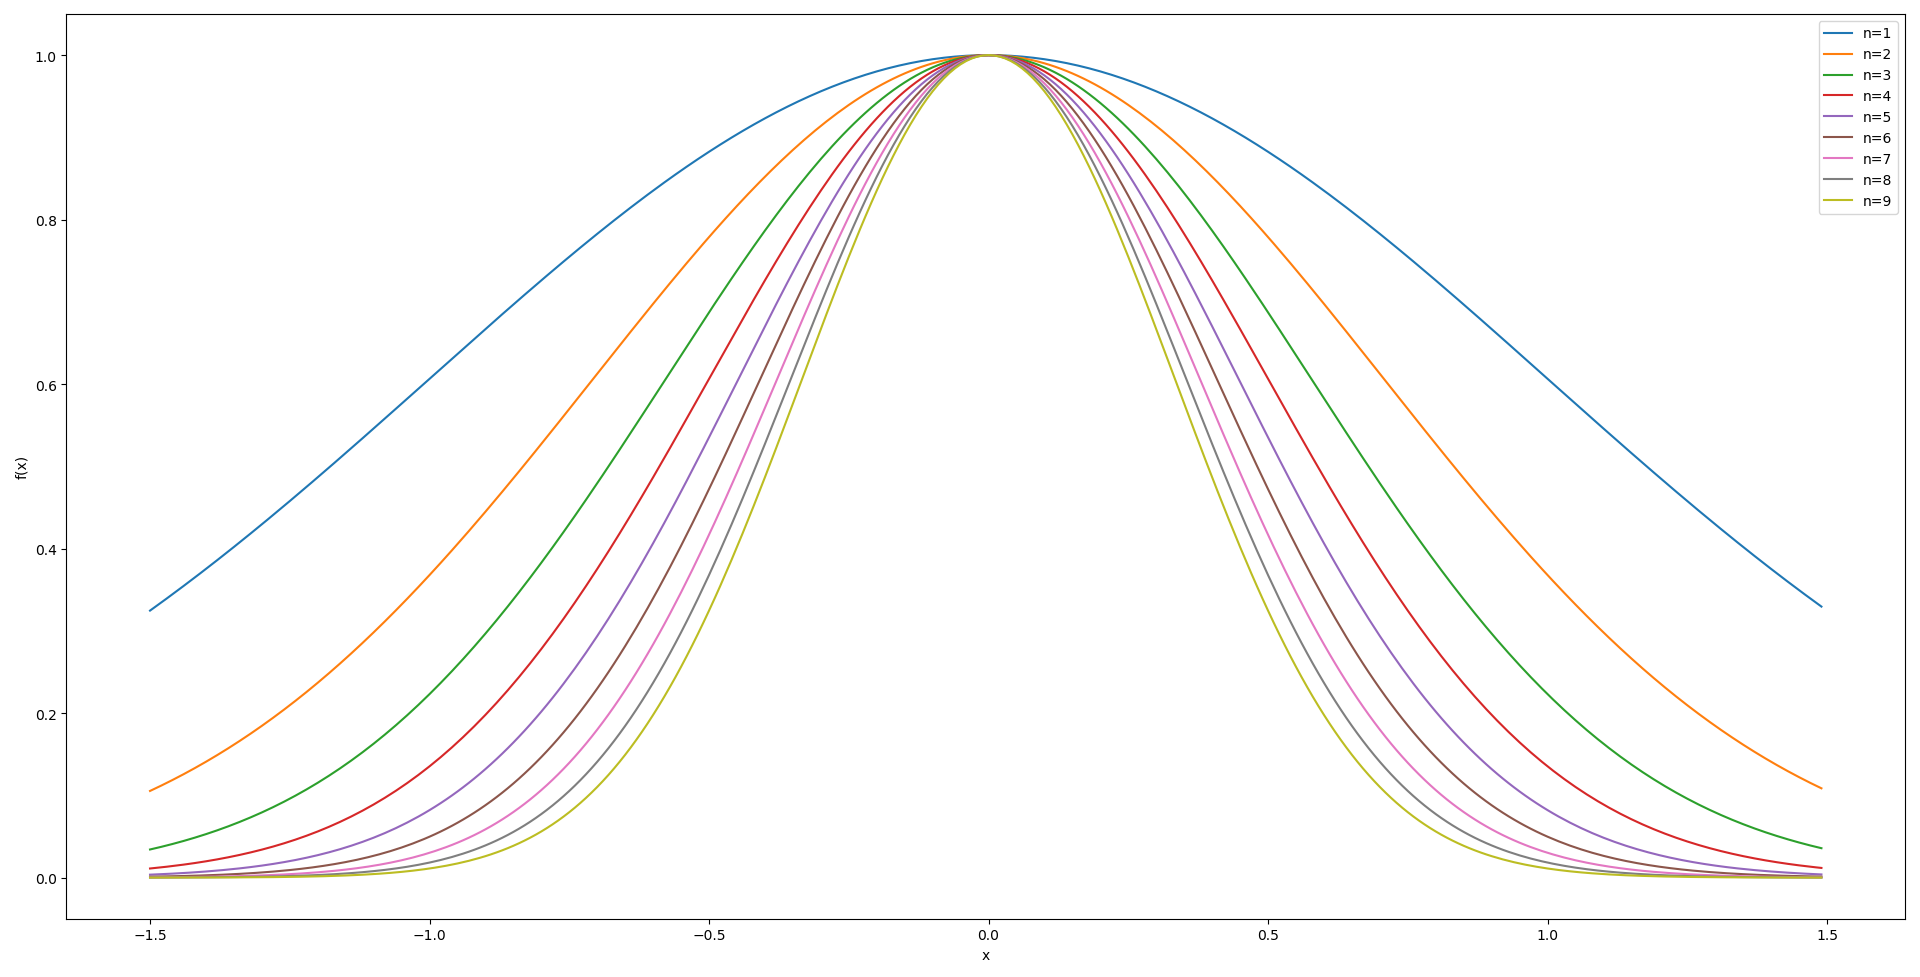
\includegraphics[width=0.5\textwidth]{STATS509/HW8/HW8Figures/problem6c.png}
    \end{center}
    \lstinputlisting[language=Python]{STATS509/HW8/HW8Code/HW8_DinoBektesevic.py}
    
    \newpage
    \item[(d)]  If we wish to perform a hypothesis test with significance level $\alpha = 0.05$, use your answer to (c) to find the values of $\bar{X}$ for which we reject $H_0$. {\it Hint: your answer should be a function of $n$.}
    
    \begin{align*}
    -2\ln{\Lambda} &= \chi^2(1) \\
    -2\ln{\left( e^{ -\frac{n}{2}\bar x^2 } \right)} &= \chi^2(x\leq 1-\alpha, 1) \\
    n\bar x^2 &= \chi^2(x\leq 1-\alpha, 1) \\
    \bar x &= \sqrt{\frac{\chi^2(x\leq 0.95, 1)}{n}} \\
    \bar x &= \frac{\sqrt{3.841458820694125958361}}{\sqrt{n}} \\
    \bar x &= \frac{1.95996}{\sqrt{n}}
    \end{align*}    
    We will reject when $\bar x$ is larger than the right hand side of the last expression.
\end{itemize}
Suppose that $n=100$ and $\bar{x}=0.16$. 
\begin{itemize}
    \item[(e)] Using your answer to (d), would we reject $H_0$ in favor of $H_1$ using significance level $\alpha=0.05$?
    
    Since $\bar x = 0.16 < \frac{1.95996}{\sqrt{100}} = 0.195996$ we would not reject.
    
    \item[(f)] Find the p-value for this hypothesis test.
    
    \begin{align*}
        p_{val} &= P(\Lambda > n\bar x^2) = 1 - \chi^2(x > n\bar x^2, 1) \\
        &= 1 - \chi^2(x \leq 100*0.0256, 1) \\
        &= 1 - \chi^2(x \leq 2.56, 1) \\
        &= 0.1096
    \end{align*}
\end{itemize}


\newpage
\subsection*{Problem 7}
A set of  times $T_1,\ldots ,T_n$ are sampled independently from a population with the following density:
$$f(t \mid \theta)  = \left\{\begin{array}{cl}
    e^{-(t-\theta)} & t \geq \theta \\
    0 & \hbox{otherwise}
    \end{array}\right.
$$
where $\theta >0$. \par
\begin{itemize}
    \item[(a)] Find the maximum likelihood estimate for $\theta$.\par
    {\it Hint: do some plots, examining the values of $\theta$ for which $f(t_1,\ldots,t_n|\theta)>0$. It may help you first to think about the cases where $n=1$ and $n=2$.  Do {\bf not}  rush into differentiating anything!}
    \item[(b)] Is there a ZES estimator for $\theta$ ? Briefly explain your answer.
\end{itemize}

\medskip
[{\bf Motivation:} (not necessary to answer the problem, but may help with intuition). For example,  the observations $T_1,\ldots , T_n$ might be the observed times taken for
$n$ messages to be transmitted across a network. In this case, 
$\theta$ represents the (non-random) minimum time for a message to be transmitted across the network if there were no delays; the additional random component of the time $(T-\theta)$ is due to bottlenecks and queues encountered by the message.]
\end{document}
